\section{Построение прямой (точки), минимально удаленной от множества плоскостей (отрезков)}\label{plane}

\subsection{Постановка задачи}\label{plane:task}

Дано множество из $n$ отрезков на плоскости или $n$ плоскостей в пространстве. Необходимо найти точку на плоскоти, минимально удаленную от заданных отрезков, или прямую в пространстве, минимально удаленную от заданных плоскостей. Меру близости на плоскости выберем равной корню из суммы квадратов расстояний от точки до прямых, содержащих отрезки. Меру близости в пространстве выберем равной корню из суммы квадратов расстояний от прямой до плоскостей: в случае параллельности или совпадения прямой и плоскости берется расстояние от любой точки прямой до плоскости, а в случае пересечения берется расстояние от плоскости до точки прямой, ближайщей к этой плоскости внутри призмы, объемлющей рассматриваемый компакт пространства. 

\begin{figure}[h]
	{ \noindent \centering
	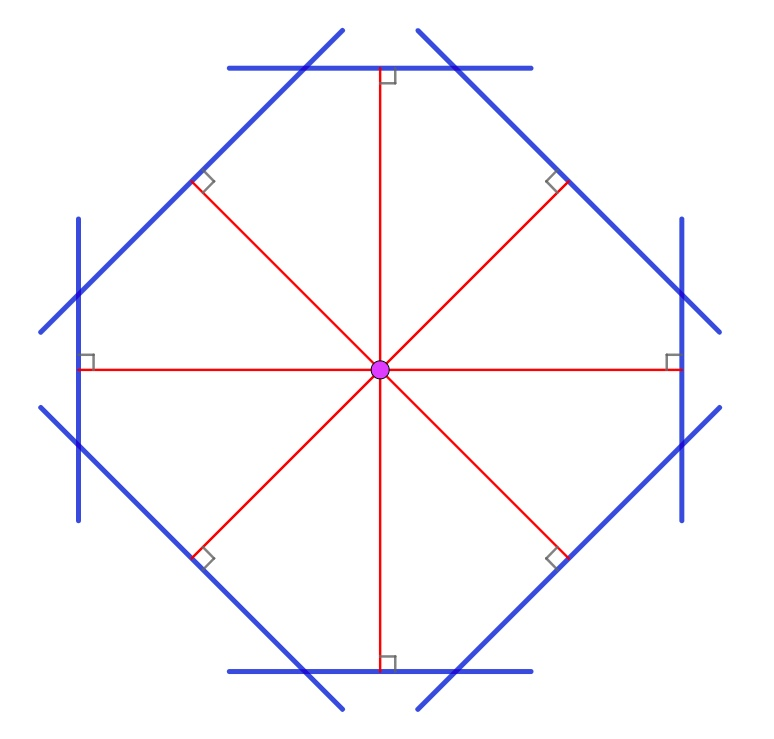
\includegraphics[scale=0.5]{plane01}
	\caption{Точка и множество отрезков на плоскости.}
	}
\end{figure}

\begin{figure}[h]
	{ \noindent \centering
	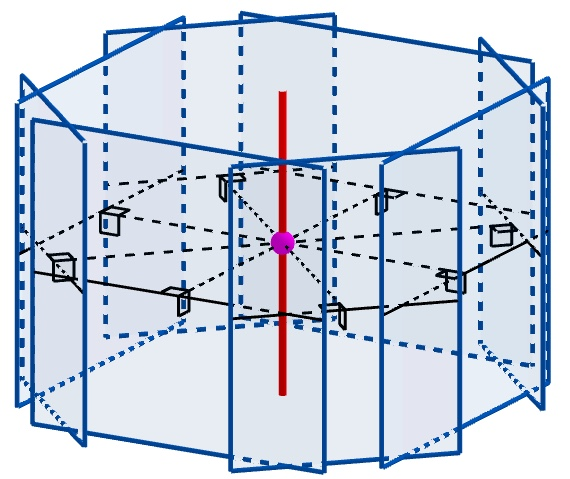
\includegraphics[scale=0.7]{plane02}
	\caption{Отрезок и множество плоскостей в пространстве.}
	}
\end{figure}

\newpage
\subsection{Двумерный случай}\label{plane:alg:2dim}

Пусть дан набор из $n-1$ отрезков в виде набора пар их вершин: 
$$S = \Set{\;((x_i, y_i), (x_{i+1}, y_{i+1}))\;}{i = \ton n-1}$$

Таким образом, у нас имеется точка, через которую проходит каждый отрезок, и направление прямой, на которой лежит каждый отрезок, и можно переписать множетсво отрезков следующим образом:
$$\begin{gathered}
	S^* =\Set{\; \left( (x_i^{(c)}, y_i^{(c)}), (l_i^x, l_i^y) \right) \;}{i= \ton n-1} \\
	x_i^{(c)} = \frac{x_i + x_{i+1}}{2}, \; y_i^{(c)} = \frac{y_i + y_{i+1}}{2} \\
	l_i^x = x_{i+1} - x_i, \; l_i^y = y_{i+1} - y_i
\end{gathered}$$

Отнормируем напрявляющие векторы прямых, содержащих отрезки:
$$\tilde{l}_i^x = \frac{x_{i+1} - x_i}{\sqrt{(x_{i+1} - x_i)^2+(y_{i+1} - y_i)^2}}, \; \tilde{l}_i^y = \frac{y_{i+1} - y_i}{\sqrt{(x_{i+1} - x_i)^2+(y_{i+1} - y_i)^2}}$$

\newpage
Тогда нормальные уравнения этих прямых будут иметь вид:

$$\begin{gathered}
	a_i x + b_i y + c_i = 0, \; i = \ton n-1 \\
	 a_i = \tilde{l}_i^y, \; b_i = -\tilde{l}_i^x, \; c_i = - (a_i x_i^{(c)} + b_i y_i^{(c)})
\end{gathered}$$

\vspace{0.5cm}
Будем искать точку $O = (x_0, y_0)$, наименее удаленную от данного множества отрезков.

Формула расстояния от точки прямой, содержащей каждый отрезок:
$$\rho (O, l_i) = \frac{|a_i x_0 + b_i y_0 + c_i|}{\sqrt{a_i^2+b_i^2}} = |a_i x_0 + b_i y_0 + c_i|, \; i = \ton n-1$$

Наша мера будет иметь вид:
$$L_0(x_0, y_0) = \sqrt{\underset{i=1}{\overset{n-1}{\sum}}(a_i x_0 + b_i y_0 + c_i)^2}$$

Будем работать не с этой меру, а с выражением под корнем (в силу монотонности функции корня это эквивалентная задача), т.е. имеем функционал:
$$L (x_0, y_0) = \underset{i=1}{\overset{n-1}{\sum}}(a_i x_0 + b_i y_0 + c_i)^2$$

Таким образом, задача свелась к поиску минимального значения выражения $L(x_0, y_0)$.

Составим систему из двух уравнений, приравняв к нулю частные производные функционала $L(x_0, y_0)$ по $x_0$ и $y_0$:
$$\begin{cases}
	\frac{\partial}{\partial x_0} \underset{i=1}{\overset{n-1}{\sum}}(a_i x_0 + b_i y_0 + c_i)^2 = \underset{i=1}{\overset{n-1}{\sum}} \left( \frac{\partial}{\partial x_0}(a_i x_0 + b_i y_0 + c_i)^2 \right) = 0 \\
	\frac{\partial}{\partial y_0} \underset{i=1}{\overset{n-1}{\sum}}(a_i x_0 + b_i y_0 + c_i)^2 = \underset{i=1}{\overset{n-1}{\sum}} \left( \frac{\partial}{\partial y_0}(a_i x_0 + b_i y_0 + c_i)^2 \right)= 0
\end{cases} \; \Leftrightarrow$$
$$\Leftrightarrow \; \begin{cases}
	\underset{i=1}{\overset{n-1}{\sum}} \left( 2 a_i (a_i x_0 + b_i y_0 + c_i) \right) = 0 \\
	\underset{i=1}{\overset{n-1}{\sum}} \left( 2 b_i (a_i x_0 + b_i y_0 + c_i) \right) = 0
\end{cases} \Leftrightarrow$$
$$ \Leftrightarrow \;  \begin{cases}
	\left( \underset{i=1}{\overset{n-1}{\sum}} a_i^2 \right) x_0 + \left( \underset{i=1}{\overset{n-1}{\sum}} a_i b_i \right) y_0 + \underset{i=1}{\overset{n-1}{\sum}} a_i c_i = 0 \\
	\left( \underset{i=1}{\overset{n-1}{\sum}} a_i b_i \right) x_0 + \left( \underset{i=1}{\overset{n-1}{\sum}} b_i^2 \right) y_0 + \underset{i=1}{\overset{n-1}{\sum}} b_i c_i = 0
\end{cases}\eqno(*)$$

Для выяснения совместности системы воспользуемся теоремой Кронекера-Капелли и следствием из нее:
\begin{theorem}[\red{Кронекера-Капелли}]\label{plane/the:1}
	Система линейных алгебраических уравнений совместна тогда и только тогда, когда ранг матрицы системы равен рангу расширенной матрицы системы, т.е. $rk A = rk \tilde{A}$
\end{theorem}

\begin{conseq}\label{plane/conseq:1}
	Из теоремы Кронекера-Капелли получаем утвреждения:
	\begin{enumerate}
		\item если $rk A \not = rk \tilde{A}$, то СЛАУ несовместна
		\item если $rk A = rk \tilde{A} < n$, то СЛАУ имеет бесконечное число решений
		\item если $rk A = rk \tilde{A} = n$, то СЛАУ имеет ровно одно решение
	\end{enumerate}
\end{conseq}

В нашем случае имеем:
$$n=2, \; A = \begin{pmatrix}
	\underset{i=1}{\overset{n-1}{\sum}} a_i^2 & \underset{i=1}{\overset{n-1}{\sum}} a_i b_i\\
	\underset{i=1}{\overset{n-1}{\sum}} a_i b_i & \underset{i=1}{\overset{n-1}{\sum}} b_i^2
\end{pmatrix}, \; \tilde{A} = \begin{pmatrix}
	\underset{i=1}{\overset{n-1}{\sum}} a_i^2 & \underset{i=1}{\overset{n-1}{\sum}} a_i b_i & -\underset{i=1}{\overset{n-1}{\sum}} a_i c_i\\
	\underset{i=1}{\overset{n-1}{\sum}} a_i b_i & \underset{i=1}{\overset{n-1}{\sum}} b_i^2 & -\underset{i=1}{\overset{n-1}{\sum}} b_i c_i
\end{pmatrix}$$

Таким образом, получаем:
\begin{itemize}
 	\item 
 		если $rk A = rk \tilde{A} = 1 < 2$, т.е. $\frac{\underset{i=1}{\overset{n-1}{\sum}} a_i^2}{\underset{i=1}{\overset{n-1}{\sum}} a_i b_i}=\frac{\underset{i=1}{\overset{n-1}{\sum}} a_i b_i}{\underset{i=1}{\overset{n-1}{\sum}} b_i^2}=\frac{\underset{i=1}{\overset{n-1}{\sum}} a_i c_i}{\underset{i=1}{\overset{n-1}{\sum}} b_i c_i}$, то система имеет бесконечное число решение, т.е. существует прямая, равноудаленная от исходного множества отрезков (прямых) - любое из уравнений системы $(*)$
 	\item 
 		если $rk A \not = rk \tilde{A} \; \Leftrightarrow \; rk A = 1, rk \tilde{A} = 2$, т.е. $\frac{\underset{i=1}{\overset{n-1}{\sum}} a_i^2}{\underset{i=1}{\overset{n-1}{\sum}} a_i b_i}=\frac{\underset{i=1}{\overset{n-1}{\sum}} a_i b_i}{\underset{i=1}{\overset{n-1}{\sum}} b_i^2}\not=\frac{\underset{i=1}{\overset{n-1}{\sum}} a_i c_i}{\underset{i=1}{\overset{n-1}{\sum}} b_i c_i}$, то система несовместна (нет решений), но это невозможно, докажем это.
 		Пусть $a = (a_1, \dots, a_{n-1}), \; b = (b_1, \dots, b_{n-1})$. Тогда матрица $A$ является матрицей скалярных произведений векторов $a$ и $b$:
 		$$A = 
 		\begin{pmatrix}
 			(a,a) & (a,b) \\
 			(a,b) & (b,b)
 		\end{pmatrix}$$
 		Из неравенства Коши-Буняковского знаем, что произведение квадратов норм векторов не меньше, чем произведение скалярных произведений этих векторов, причем равенство достигается, только если векторы пропорциональны. Таким образом, если они не пропорциональны, то $rk A = rk \tilde{A} = 2$, а если пропорциональны, то $rk A = rk \tilde{A} = 1$, т.е. случай $rk A \not = rk \tilde{A}$ невозможен.
 	\item
 		если $rk A = rk \tilde{A} = 2$, т.е. $\begin{vmatrix}
			\underset{i=1}{\overset{n-1}{\sum}} a_i^2 & \underset{i=1}{\overset{n-1}{\sum}} a_i b_i\\
			\underset{i=1}{\overset{n-1}{\sum}} a_i b_i & \underset{i=1}{\overset{n-1}{\sum}} b_i^2
		\end{vmatrix} \not = 0$, то система имеет единственное решение (одну точку):
		$$\begin{cases}
		x_0 = \frac{\left( \underset{i=1}{\overset{n-1}{\sum}} b_i^2 \right) \left( \underset{i=1}{\overset{n-1}{\sum}} a_i c_i \right) - \left( \underset{i=1}{\overset{n-1}{\sum}} a_i b_i \right) \left( \underset{i=1}{\overset{n-1}{\sum}} b_i c_i \right)}{\left( \underset{i=1}{\overset{n-1}{\sum}} a_i b_i \right)^2 - \left( \underset{i=1}{\overset{n-1}{\sum}} a_i^2 \right)\left( \underset{i=1}{\overset{n-1}{\sum}} b_i^2 \right)} \\
		y_0 = \frac{\left( \underset{i=1}{\overset{n-1}{\sum}} a_i^2 \right) \left( \underset{i=1}{\overset{n-1}{\sum}} b_i c_i \right) - \left( \underset{i=1}{\overset{n-1}{\sum}} a_i b_i \right) \left( \underset{i=1}{\overset{n-1}{\sum}} a_i c_i \right)}{\left( \underset{i=1}{\overset{n-1}{\sum}} a_i b_i \right)^2 - \left( \underset{i=1}{\overset{n-1}{\sum}} a_i^2 \right)\left( \underset{i=1}{\overset{n-1}{\sum}} b_i^2 \right)}
	\end{cases}$$
 \end{itemize}

\newpage
\subsection{Трехмерный случай}\label{plane:alg:3dim}

\subsubsection{Случай параллельности плоскостей и прямой}\label{plane:alg:3dim:paral}

Пусть дан набор из $n$ плоскостей в виде набора пар их векторов нормали и точек, принадлежащих им: 
$$S = \Set{\;((x_i, y_i, z_i), (m_i, n_i, p_i))\;}{i = \ton n}$$

По смыслу задачи координата $l_i$ для всех плоскостей равна 0, или существует афинная замена координат, приводящая к такой ситуации, т.е. пользуемся алгоритмом замены координат \ref{coords:alg:3dim}. Таким образом, имеем следующий набор:
$$S = \Set{\;((x_i, y_i, z_i), (m_i, n_i, 0))\;}{i = \ton n}$$

Отнормируем вектора нормали плоскостей:
$$\tilde{m_i} = \frac{m_i}{\sqrt{m_i^2+n_i^2}}, \; \tilde{n_i} = \frac{n_i}{\sqrt{m_i^2+n_i^2}}$$

Тогда уравнения наших плоскостей имеют вид:
$$\tilde{m_i} (x - x_i) + \tilde{n_i} (y - y_i) = 0$$

Если рассматривать обычное уравнение плоскости, то получаем следующие тождества:
$$\begin{gathered}
	A x + B y + C z + D = 0 \\
	A = \tilde{m_i}, \; B = \tilde{n_i}, \; C = 0, \; D = -\tilde{m_i} x_i - \tilde{n_i} y_i
\end{gathered}$$

Будем искать прямую $l$, наименее удаленную от данного множества плоскостей:
\begin{center}
	$\mathit{l}: \; \begin{cases}
		x = x_0 + m \cdot t \\
		y = y_0 + n \cdot t \\
		z = z_0 + p \cdot t
	\end{cases}$, где $t \in \mathbb{R}$ - параметр. 
\end{center}

Т.к. все плоскости параллельны оси OZ, то и искомая прямая будет параллельна ей, т.е. направляющий вектор будет равен $(0,0,1)$. Таким образом, задача свелась к нахождению точки, наименее удаленной от множества данных плоскостей, в любой плоскости, например, $z = 0$. В пересечении плоскости $z=0$ и исходного набора плоскостей получаем набор отрезков (прямых), и задача полностью свелась к двумерному случаю \ref{plane:alg:2dim}.

\subsubsection{Случай непараллельности плоскостей и прямой}\label{plane:alg:3dim:neparal}

Аналогично случаю параллельности \ref{plane:alg:3dim:paral} имеем нормальные уравнения плоскостей:
$$\begin{gathered}
	\pi_i: \; A_i x + B_i y + C_i z + D_i = 0 \\
	A_i = \frac{m_i}{\sqrt{m_i^2 + n_i^2 + p_i^2}}, \;
	B_i = \frac{n_i}{\sqrt{m_i^2 + n_i^2 + p_i^2}} \\
	C_i = \frac{p_i}{\sqrt{m_i^2 + n_i^2 + p_i^2}}, \;
	D_i = -\frac{m_i x_i + n_i y_i + p_i z_i}{\sqrt{m_i^2 + n_i^2 + p_i^2}}
\end{gathered}$$

Будем рассматривать задачу внутри объемлющей призмы, ограниченной $z_{min}$ и $z_{max}$, т.е. концы искомого отрезка будем искать на этих плоскостях, ограничивающий призму <<сверху>> и <<снизу>>. Наша прямая будет определяться точками $P_1 = (x_1, y_1, z_{min})$ и $P_2 = (x_2, y_2, z_{max})$.\\

% Одну из точек прямой можно зафиксировать. Найдем среднее значение $z_{mid}$ среди всех диапазона значений $z$. Проведем плоскость, параллельную плоскости OXY: $z = z_{mid}$. В пересечении этой плоскости с исходными имеем прямые, решаем двумерную задачу нахожения точки, наименее удаленной от прямых \ref{plane:alg:2dim}.

Будем искать расстояние от прямой до каждой их плоскостей следующим образом: пусть $d_1 = \rho \left( P_1, \pi_i \right), \;\; d_2 = \rho \left( P_2, \pi_i \right)$, тогда $\rho (l, \pi_i) = \frac{d_1^2 + d_2^2 + d_1 d_2}{3}$.\\

$$\begin{gathered}
	d_{1i} = \rho \left( P_1, \pi_i \right) = |A_i x_1 + B_i y_1 + C_i z_{min} + D_i| \\
	d_{2i} = \rho \left( P_2, \pi_i \right) = |A_i x_2 + B_i y_2 + C_i z_{max} + D_i|\\
	\rho (l, \pi_i) = \frac{d_1^2 + d_2^2 + d_1 d_2}{3} = \\
	= \frac{\left( A_i x_1 + B_i y_1 + C_i z_{min} + D_i \right)^2 + \left( A_i x_2 + B_i y_2 + C_i z_{max} + D_i \right)^2}{3} + \\
	+ \frac{|A_i x_1 + B_i y_1 + C_i z_{min} + D_i||A_i x_2 + B_i y_2 + C_i z_{max} + D_i|}{3}
\end{gathered}$$

В плоскостях $z = z_{min}$ и $z = z_{max}$ будем искать точки $P_1$ и $P_2$ так, чтобы они были наименее удалены от исходных плоскостей $\pi_i$.

$$d_{ji} = \rho \left( P_1, \pi_i \right) = |A_i x_j + B_i y_j + C_i z_j + D_i|, \;\; j = 1,2, \;\; z_j = \begin{cases}
	z_{min}, \; j = 1 \\
	z_{max}, \; j = 2
\end{cases}$$

Тогда функционал имеет вид:
$$\Lambda = \underset{i=1}{\overset{n}{\sum}}(A_i x_j + B_i y_j + C_i z_{min} + D_i)^2$$

Найдем частные производные функционала по $x_j$ и $y_j$:
$$\begin{cases}
	\frac{\partial}{\partial x_j} \underset{i=1}{\overset{n}{\sum}}(A_i x_j + B_i y_j + C_i z_j + D_i)^2 = 0 \\
	\frac{\partial}{\partial y_j} \underset{i=1}{\overset{n}{\sum}}(A_i x_j + B_i y_j + C_i z_j + D_i)^2 = 0
\end{cases}\; \Rightarrow \; $$
$$\begin{gathered}
	\begin{cases}
		\underset{i=1}{\overset{n}{\sum}}\frac{\partial}{\partial x_j}(A_i x_j + B_i y_j + C_i z_j + D_i)^2 = 0 \\
		\underset{i=1}{\overset{n}{\sum}}\frac{\partial}{\partial y_j}(A_i x_j + B_i y_j + C_i z_j + D_i)^2 = 0
	\end{cases} \Rightarrow \; 
	\begin{cases}
		\underset{i=1}{\overset{n}{\sum}}2A_i (A_i x_j + B_i y_j + C_i z_j + D_i) = 0 \\
		\underset{i=1}{\overset{n}{\sum}}2B_i (A_i x_j + B_i y_j + C_i z_j + D_i) = 0
	\end{cases}\\
	\; \Rightarrow \begin{cases}
		\left( \underset{i=1}{\overset{n}{\sum}} A_i^2 \right) x_j + \left( \underset{i=1}{\overset{n}{\sum}} A_i B_i \right) y_j + \underset{i=1}{\overset{n}{\sum}}A_i (C_i z_j + D_i) = 0 \\
		\left( \underset{i=1}{\overset{n}{\sum}} A_i B_i \right) x_j + \left( \underset{i=1}{\overset{n}{\sum}} B_i^2 \right) y_j + \underset{i=1}{\overset{n}{\sum}}B_i (C_i z_j + D_i) = 0
	\end{cases}
\end{gathered}$$

Введем обозначения:
$$\begin{cases}
	a_{11} = \underset{i=1}{\overset{n}{\sum}} A_i^2 \\
	a_{12} = \underset{i=1}{\overset{n}{\sum}} A_i B_i \\
	a_{22} = \underset{i=1}{\overset{n}{\sum}} B_i^2 \\
	b_1 = \underset{i=1}{\overset{n}{\sum}}A_i (C_i z_j + D_i) \\
	b_2 = \underset{i=1}{\overset{n}{\sum}}B_i (C_i z_j + D_i)
\end{cases}$$

Если система невырождена, то получаем решение:
$$\begin{cases}
	x_j = \frac{a_{22} b_1 - a_{12} b_2}{a_{12}^2 - a_{11}a_{22}} \\
	y_j = \frac{a_{11} b_2 - a_{12} b_1}{a_{12}^2 - a_{11}a_{22}}
\end{cases}$$

Таким образом, имеем две точки, по которым однозначно определяется искомая прямая.

% \newpage
% \subsection{Примеры работы программ}\label{plane:application}

% \subsubsection{Двумерный случай}\label{plane:application:2dim}

% ждет заполнения

% \newpage
% \subsubsection{Трехмерный случай}\label{plane:application:3dim}

% ждет заполнения